\documentclass[varwidth=40cm]{standalone}
\usepackage{tikz}
\usepackage{style}

\let\r\undefined
\newcommand{\r}[1]{\draw[fill=lightgray] (#1,0) rectangle (#1+1,1);}

\begin{document}
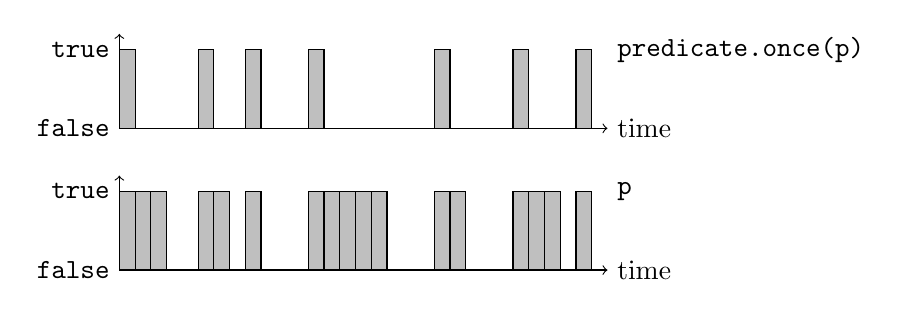
\begin{tikzpicture}[xscale=0.2]
  \r{0}
  \r{1}
  \r{2}
  \r{5}
  \r{6}
  \r{8}
  \r{12}
  \r{13}
  \r{14}
  \r{15}
  \r{16}  
  \r{20}
  \r{21}
  \r{25}
  \r{26}
  \r{27}
  \r{29}
  \draw[->] (0,0) -- (31,0) node[right] {time};
  \draw[->] (0,0) -- (0,1.2);
  \draw (0,0) node[left] {\texttt{false}};
  \draw (0,1) node[left] {\texttt{true}};
  \draw (31,1) node [right] {\texttt{p}};
  \begin{scope}[shift={(0,1.8)}]
    \r{0}
    \r{5}
    \r{8}
    \r{12}
    \r{20}
    \r{25}
    \r{29}
    \draw[->] (0,0) -- (31,0) node[right] {time};
    \draw[->] (0,0) -- (0,1.2);
    \draw (0,0) node[left] {\texttt{false}};
    \draw (0,1) node[left] {\texttt{true}};
    \draw (31,1) node [right] {\texttt{predicate.once(p)}};
  \end{scope}
\end{tikzpicture}
\end{document}
